
\documentclass[conference]{IEEEtran}
\usepackage{blindtext, graphicx}
\usepackage[super,square]{natbib}



\begin{document}
\title{Scalability of Hadoop Framework}

\author{\IEEEauthorblockN{Ayush Shakya}
\IEEEauthorblockA{Deparment of Electronics and\\Computer Engineering\\
Institute of Engineering,\\
Pulchowk, Lalitpur\\
Email: }
\and
\IEEEauthorblockN{Bijay Gurung}
\IEEEauthorblockA{Deparment of Electronics and\\Computer Engineering\\
Institute of Engineering,\\
Pulchowk, Lalitpur\\
Email:}
\and
\IEEEauthorblockN{Mahendra Singh Thapa}
\IEEEauthorblockA{Deparment of Electronics and\\Computer Engineering\\
Institute of Engineering,\\
Pulchowk, Lalitpur\\
Email:}
\and
\IEEEauthorblockN{Mehang Rai}
\IEEEauthorblockA{Deparment of Electronics and\\Computer Engineering\\
Institute of Engineering,\\
Pulchowk, Lalitpur\\
Email: mehang.rai007@gmail.com}
}

\maketitle
\begin{abstract}
        Written at last.
\end{abstract}
% Note that keywords are not normally used for peerreview papers.
\begin{IEEEkeywords}
        Hadoop, scalability, distributed system, MapReduce.
\end{IEEEkeywords}

\IEEEpeerreviewmaketitle



\section{Introduction}
Apache Hadoop is an open-source software framework for distributed storage
and distributed processing of very large data sets on computer clusters built from commodity
hardware.\cite{Apache} Hadoop is an Apache top-level project being built and used by a global
community of contributors and users. It is licensed under the Apache License 2.0.\cite{Introapache} 
Hadoop was created by Doug Cutting and Mike Cafarella in 2005.
\par The Hadoop framework is mostly written in Java programming language,
with some native code in C programming language and command line utilities
written as shell scripts. Though MapReduce Java code is common, any programming language can
be used with “Hadoop Streaming” to implement the “map” and “reduce” parts of the user’s program.\cite{Hadoopadventures}
Other projects in the Hadoop ecosystem expose richer user interfaces.
All the modules in Hadoop are designed with a fundamental assumption that
hardware failures are common and should be automatically handled by the framework.
It provides massive storage for any kind of data, enormous processing power and the ability to handle virtually
limitless concurrent tasks or jobs.
\par Some key features of Hadoop are:
\begin{enumerate}
        \item \textbf{Ability to store and process huge amounts of any kind of data quickly:}
                With data volumes and varieties constantly increasing, especially from social media and the Internet of Things(IoT), that’s a key consideration.
        \item \textbf{Computing power:} Hadoop’s distributed computing model processes big data fast. The more computing nodes you use, the more processing power you have.
        \item \textbf{Fault tolerance:} Data and application processing are protected against hardware failure. If a node goes down, jobs are automatically redirected to other nodes to make sure the distributed computing does not fail. Multiple copies of all data are stored automatically.
        \item \textbf{Flexibility:} Unlike traditional relational databases, you don’t have to preprocess data before storing it. You can store as much data as you want and decide how to use it later. That includes unstructured data like text, images and videos.
        \item \textbf{Low cost:} The open-source framework is free and uses commodity hardware to store large quantities of data.
        \item \textbf{Scalability:} You can easily grow your system to handle more data simply by adding nodes. Little administration is required.
\end{enumerate}
\par Since unstructured data are quite complex and voluminous as they come from a variety
of sources, such as emails, text documents, videos, photos, audio files,etc., traditional
database cannot handle them. In such case, hadoop’s ability to join, aggregate, and analyze
vast stores of multi-source data without having to structure it first allows organizations to
gain deeper insights quickly. But hadoop must not be confused as a database. You can easily grow your system to handle more data simply by adding nodes. Little administration is required.
\par Hadoop makes it possible to run applicaitons on systems with thousands of nodes involving thousands of terabytes. It's distributed file system facilities rapid
data transfer rates among nodes and allows the system to continue operating uninterrupted in case of a node failure. This approach lowers the risk of catastrphic system failure,
even if a significant number of nodes become inoperative.

\section{History of Hadoop}
As the World Wide Web grew in the late 1900s and early 2000s, search engines and indexes were created to help locate relevant information amid the text-based content. In the early years, search results were returned by humans. But as the web grew from dozens to millions of pages, automation was needed. Web crawlers were created, many as university-led research projects, and search engine start-ups took off (Yahoo, AltaVista, etc.).
\par One such project was an open-source web search engine called Nutch – the brainchild of Doug Cutting and Mike Cafarella. They wanted to return web search results faster by distributing data and calculations across different computers so multiple tasks could be accomplished simultaneously. During this time, another search engine project called Google was in progress. It was based on the same concept – storing and processing data in a distributed, automated way so that relevant web search results could be returned faster.
\par In 2006, Cutting joined Yahoo and took with him the Nutch project as well as ideas based on Google’s early work with automating distributed data storage and processing which was published in October 2003. This paper spawned another research paper from Google - MapReduce: Simplified Data Processing on Large Clusters in December, 2004. The Nutch project was divided – the web crawler portion remained as Nutch and the distributed computing and processing portion became Hadoop (named after Cutting’s son’s yellow plush toy elephant). In 2008, Yahoo released Hadoop as an open-source project. The initial code that was factored out of Nutch consisted of 5k lines of code for NDFS and 6k lines of code for MapReduce. Today, Hadoop’s framework and ecosystem of technologies are managed and maintained by the non-profit Apache Software Foundation (ASF), a global community of software developers and contributors.
\par The first committer added to the Hadoop project was Owen O’Malley in March 2006. Hadoop 0.1.0 was released in April 2006 and continues to evolve by the many contributors to the Apache Hadoop project.
\par Yahoo started using Hadoop on a 1000 node cluster. Then on january 2008, Apache took over Hadoop. In July 2008, 4000 node cluster were tested successfully with Hadoop. Hadoop successfully sorted a petabyte
of data in less than 17 hours to handle billions of searches and indexing millions of web pages.
Until this date, several version of Hadoop has been released. The latest version of Hadoop is version 2.7 which was released on June 2015.
\par Since Hadoop is an open-source so many popular company has contributed to it. With the likes of Google and Yahoo being already involved in it's early
development, there are popular companies like Facebook, eBay, etc. are contributing to it. On January 2011, Facebook, LinkedIn, eBay and IBM collectively contributed 200,000 lines of code. By June 2011, Yahoo had 
42k Hadoop nodes and hundreds of petabytes of storage.\cite{Wikiapache}
\par Cloudera was founded in 2008 to commercialize Apache Hadoop, with an awareness of three key trends that are changing the way the entire industry stores and uses data. These changes came first to consumer Internet properties, but loom large or commercial, defense, and
intelligence applicaitons as well.

\section{Overview of Technologies}
The core of Apache Hadoop consists of a storage part, known as Hadoop Distributed File System (HDFS), and a processing part called MapReduce. Hadoop splits files into large blocks and distributes them across nodes in cluster. To process data, Hadoop transfers packaged code for nodes to process in parallel
based on the data that needs to be processed. This approach takes advantage of data locality - nodes manipulating tha data they have access to - to allow the dataset to be processes faster and more efficiently than it would be in a more conventional supercomputer architecture that relies on a parallel file 
system where computation and data are distributed via high-speed networking.
\par The base Apache Hadoop framework is composed of the following modules:
\begin{enumerate}
        \item \textbf{Hadoop Common:}
                It contains libraries and utilities needed by other Hadoop modules.
        \item \textbf{Hadoop Distributed File System (HDFS):}
It is a distributed file-system that stores data on commodity machines, providing very high aggregate bandwidth across the cluster.
It is one of the primary components at the core of Apache Hadoop 1.x. It is an open source projects, inspired by technologies created inside Google.
\begin{figure}[h!]
        \centering
        \includegraphics[width=80mm]{hdfs}
        \caption{Architecture of Hadoop distributed file system}
\end{figure}
The Hadoop distributed file system (HDFS) is a distributed, scalable, and portable file-system written in 
Java for the Hadoop framework. Each node in a Hadoop instance typically has a single namenode, and a cluster
of datanodes form the HDFS cluster. The situation is typical because each node does not require a datanode
to be present. Each datanode serves up blocks of data over the network using a block protocol specific to
HDFS. The file system uses the TCP/IP layer for communication. Clients use Remote procedure call (RPC) to
communicate between each other.\\
\par HDFS stores large files (typically in the range of gigabytes to terabytes) across multiple machines. It achieves reliability by replicating the data across multiple hosts, and hence does not require RAID storage on hosts. With the default replication value, 3, data is stored on three nodes: two on the same rack, and one on a different rack. Data nodes can talk to each other to rebalance data, to move copies around, and to keep the replication of data high. HDFS is not fully POSIX-compliant, because the requirements for a POSIX file-system differ from the target goals for a Hadoop application. The tradeoff of not having a fully POSIX-compliant file-system is increased performance for data throughput and support for non-POSIX operations such as Append.
\par The HDFS file system includes a so-called secondary namenode, which misleads some people into thinking that when the primary namenode goes offline, the secondary namenode takes over. In fact, the secondary namenode regularly connects with the primary namenode and builds snapshots of the primary namenode's directory information, which the system then saves to local or remote directories. These checkpointed images can be used to restart a failed primary namenode without having to replay the entire journal of file-system actions, then to edit the log to create an up-to-date directory structure. Because the namenode is the single point for storage and management of metadata, it can become a bottleneck for supporting a huge number of files, especially a large number of small files. HDFS Federation, a new addition, aims to tackle this problem to a certain extent by allowing multiple name-spaces served by separate namenodes.
\par An advantage of using HDFS is data awareness between the job tracker and task tracker. The job tracker schedules map or reduce jobs to task trackers with an awareness of the data location.
This reduces the amount of traffic that goes over the network and prevents unnecessary data transfer. When Hadoop is used with other file systems, this advantage is not always available. This can have a significant impact on job-completion times, which has been demonstrated when running data-intensive jobs. HDFS was designed for mostly immutable files and may not be suitable for systems requiring concurrent write-operations.
\par Another limitation of HDFS is that it cannot be mounted directly by an existing operating system. Getting data into and out of the HDFS file system, an action that often needs to be performed before and after executing a job, can be inconvenient. A filesystem in Userspace (FUSE) virtual file system has been developed to address this problem, at least for Linux and some other Unix systems.
\par File access can be achieved through the native Java API, the Thrift API, to generate a client in the language of the users' choosing (C++, Java, Python, PHP, Ruby, Erlang, Perl, Haskell, C\#, Cocoa, Smalltalk, or OCaml), the command-line interface, or browsed through the HDFS-UI web app over HTTP.

        \item \textbf{Hadoop MapReduce:}
                It is an implementation of the MapReduce programming model for large scale data processing
It is one of the primary components at the core of Apache Hadoop 1.x. It is an open source projects, inspired by technologies created inside Google.
\begin{figure}[h!]
        \centering
        \includegraphics[width=80mm]{mapreduce}
        \caption{Architecture of Hadoop distributed file system}
\end{figure}
With Hadoop distributed file system comes the MapReduce engine, which consists of one JobTracker, to which client applications submit MapReduce jobs.
The JobTracker pushes work out to available TaskTracker nodes in the cluster, striving to keep the work as close to the data as possible.
\par With a rack-aware file system, the JobTracker knows which node contains the data, and which other machines are nearby. If the work cannot be hosted on the actual node where the data resides, priority is given to nodes in the same rack. This reduces network traffic on the main backbone network.
\par If a TaskTracker fails or times out, that part of the job is rescheduled. The TaskTracker on each node spawns off a separate Java Virtual Machine process to prevent the TaskTracker itself from failing if the running job crashes the JVM. A heartbeat is sent from the TaskTracker to the JobTracker every few minutes to check its status. The Job Tracker and TaskTracker status and information is exposed by Jetty and can be viewed from a web browser.
\par If the JobTracker failed on Hadoop 0.20 or earlier, all ongoing work was lost. Hadoop version 0.21 added some checkpointing to this process. The JobTracker records what it is up to in the file system. When a JobTracker starts up, it looks for any such data, so that it can restart work from where it left off.
\par MapReduce programming is not a good match for all problems. It’s good for simple information requests and problems that can be divided into independent units, but it's not efficient for iterative and interactive analytic tasks. MapReduce is file-intensive. Because the nodes don’t intercommunicate except through sorts and shuffles, iterative algorithms require multiple map-shuffle/sort-reduce phases to complete. This creates multiple files between MapReduce phases and is inefficient for advanced analytic computing.

        \item \textbf{Hadoop YARN:}
            YARN (Yet Another Resource Negotiator) is Hadoop’s cluster resource management
system. YARN was introduced in Hadoop 2.0 to improve the MapReduce implementation,
but it is general enough to support other distributed computing paradigms
as well.\\

The fundamental idea of YARN is to split up the two major responsibilities of the JobTracker,
in other words resource management and job scheduling/monitoring, into separate daemons: a
global ResourceManager and per-application ApplicationMaster (AM). The ResourceManager
and per-node slave, the NodeManager (NM), form the new, and \textit{generic}, operating system for
managing applications in a distributed manner. 

The ResourceManager is the ultimate authority that arbitrates resources among all the
applications in the system. The per-application ApplicationMaster is, in effect, a \textit{framework
specific} entity and is tasked with negotiating resources from the ResourceManager and working
with the NodeManager(s) to execute and monitor the component tasks.

The ResourceManager has a pluggable scheduler component, which is responsible for
allocating resources to the various running applications subject to familiar constraints of
capacities, queues etc. The Scheduler is a \textit{pure scheduler} in the sense that it performs no
monitoring or tracking of status for the application, offering no guarantees on restarting failed
tasks either due to application failure or hardware failures. The scheduler performs its
scheduling function based on the \textit{resource requirements} of an application by using the abstract
notion of a \textit{resource container}, which incorporates resource dimensions such as memory, CPU,
disk, network etc. 

The NodeManager is the per-machine slave, which is responsible for launching the
applications’ containers, monitoring their resource usage (CPU, memory, disk, network), and
reporting the same to the ResourceManager. 

The per-application ApplicationMaster has the responsibility of negotiating appropriate
resource containers from the Scheduler, tracking their status and monitoring for progress. From
the system perspective, the ApplicationMaster itself runs as a normal \textit{container}.

\begin{figure}[h!]
        \centering
        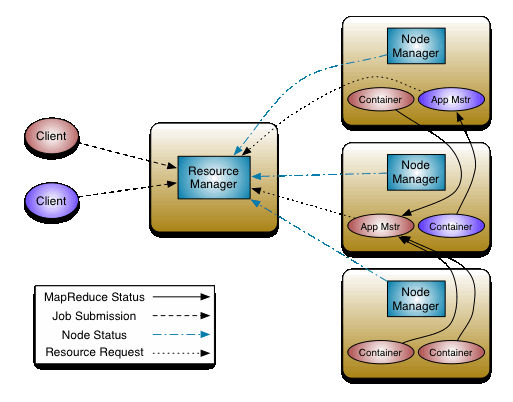
\includegraphics[width=80mm]{yarn}
        \caption{Architectural view of YARN}
\end{figure}

One of the crucial implementation details for MapReduce within the new YARN system is the
reuse of the existing MapReduce framework without any major surgery. This step was very
important to ensure compatibility for existing MapReduce applications and users. 


\end{enumerate}


\section{Hadoop And Scalability}

\subsection{A word on Scalability}

Scalability is difficult to define. \cite{Hill1990} Mostly because, while it is valued, its characteristics and
the characteristics that undermine it are usually only apparent from the context. However,
we can say that Scalability is the capability of a system, network, or process to handle a
growing amount of work, or its potential to be enlarged in order to accommodate that
growth. \cite{Bondi2000}

Consequently, a system whose performance improves after adding hardware,
proportionally to the capacity added, is said to be a scalable system.

Scalability can be distinguished based on the methods used to achieve it:

Horizontal scaling also referred to as “scale out” means that we scale by adding more
machines into our pool of resources.
Vertical scaling or “scale up” means that we scale by adding more power (CPU, RAM) to
our existing machine.

\subsection{Scalability in Hadoop}

Hadoop achieves scalability by scaling out. We can add new nodes as necessary and without needing to change data formats, data loading procedures, how jobs are written, or the applications on top.

So, the idea behind Hadoop is to provide scalability through the ability to use cheap commodity clusters on a distributed file system. 
Also, the inexpensive servers run on parallel. 

So, almost all the features of Hadoop contribute to its scalability:

\begin{itemize}

    \item \textbf{Cost-Effectiveness:} Hadoop reduces the cost of processing huge amounts of data by making use of cheap, commodity hardware. 
            It is not necessary to invest heavily on high-end servers and machines. 
            This cost-effectiveness means that it is easier to scale.

    \item \textbf{Flexibility:} Hadoop accepts any type of data, structured or not, as long as they can be stored in a file. 
            It is schema-less and can join data arbitrarily from multiple sources. 
            So, the traditional Extract Load Transform (ETL) process can be avoided. 
            This is the better approach when handling large amounts of data during the scaling process.

   \item \textbf{Fault-tolerance:} When a node goes down, the system automatically redirects work to another location of the same data. 
       This type of fault-tolerance is crucial when the amount of data and possibilities of failures grow when scaling.

\end{itemize}

\subsection{Limitations on Scalability in Hadoop 1.x and their solutions in Hadoop 2.x}

\textbf{Namenode as the single point of failure}

The namenode (the dedicated server that maintains the namespace) is the single point of failure in Hadoop 1.x 
and the ability to scale is hampered by its memory as it keeps the entire namespace in RAM. 
So, as the number of data nodes increases, the high load on the single centralized namenode server means 
that the performance and availability of the clusters are hampered, eventually affecting the overall scalability. 
Thus, the scalability of the overall system is held back by the scalability of the namenode \cite{Shvachko2010}, especially in 
cases where the files are generally small in size and numerous. Even if the system could scale horizontally, the 
namenode could only scale vertically. 

Also, the collocation of namespace and block management in the namenode meant that the two layers were too coupled. 

In the Yahoo! Paper describing the HDFS \cite{Shvachko2010b}, the authors acknowledged this problem and described their near term 
solution of “allowing multiple namespaces (and NameNodes) to share the physical storage within a cluster”.

However, multiple namespaces have the drawback of the additional burden of actually managing them. 

Still, many proposed solutions used multiple namespaces in one form or the other. \cite{Singh2012}

Hadoop 2.x tackled this issue by introducing features such as the Hadoop Federation.

\begin{figure}[h!]
        \centering
        \includegraphics[width=80mm]{HDFS_Federation}
        \caption{HDFS Federation Architecture}
\end{figure}

Federation makes use of multiple namenodes/namespaces that are federated meaning they are independent and do not 
require coordination with each other. The datanodes are used as common storage for blocks by all the namenodes. 
Each datanode registers with all the namenodes in the cluster. Datanodes send periodic heartbeats and block reports 
and handles commands from the namenodes.\cite{Suresh2011}

\textbf{Overburdened JobTracker}

In Hadoop 1.0, there is tight coupling between Cluster Resource Management and MapReduce programming model. 
Job Tracker, which does resource management, is part of the MapReduce Framework. 
This limits the scalability as the Job Tracker is running on a single machine doing a variety of activities like 
resource management, job and task scheduling, monitoring, etc while a lot of machines (the datanodes) are not utilized fully.

Hadoop 2.x solved this issue by introducing YARN which splits the two major functionalities of Job Tracker—resource 
management and job scheduling/monitoring into two separate components: Resource manager and Node Manager. 
YARN also took over the task of cluster management from MapReduce so that MapReduce is streamlined to only perform Data Processing.

\textbf{Limitation in running non-MapReduce Application}

Another of the ill-effects of Job tracker’s tight integration with MapReduce in Hadoop 1.0 is that only supporting application 
that obeys MapReduce programming framework can run on Hadoop. 

This is a problem as MapReduce is not always the best choice of programming paradigm. 
For instance, in cases like real-time analysis, message-passing between processes, running Ad-hoc query, etc, 
MapReduce performs badly or cannot do them altogether. So, systems that would require services like these when scaling 
would be held back by Hadoop. 

Again, Hadoop 2.x solves it with YARN as it decouples the resource management and data processing part of MapReduce. 
Thus, it allows other distributed computing models like Spark, Hama, Giraph, MPI (Message Passing Interface) and HBase 
coprocessors to work with Hadoop. 

\section{Future of Hadoop}

It is forecasted that the global Hadoop market value will reach \$50.2 billion 
by 2020. In the next few years, more enterprises will adopt a data-driven 
business and will look to Hadoop to support their growth. Hadoop will allow 
for leaner, faster and more efficient enterprises. The focus on Hadoop will 
also create opportunities for new entrants in the market, to rise to and solve 
its challenges. In future, Hadoop will be used by world-class enterprises, 
as well as businesses of all sizes for managing, processing and leveraging 
data to better serve their customers.

\subsection{Hadoop will Power the Connected World}
As each company connects to various partners, customers, vendors and things,
the ocean of data grows and becomes intertwined with data lakes and rivers. 
Hadoop will power this connected world and it will be used to address
uses cases that require a mix of batch, real-time, streaming and interactive 
scenarios.

\subsection{Hadoop Will Be Used for Processing and Storing Highly Sensitive Data}
The lack of built-in security in Hadoop is an obstacle that enterprises face 
today, but new tools are emerging that address this issue, connecting Kerberos 
and MapReduce components and ensuring compatibility between data. In Future, 
expect these issues to resolved and highly regulated organizations to be managing their secure data with Hadoop.

\subsection{Hadoop Will Advance the Internet of Things}
The Internet of things is only possible with instant data processing and prescriptive analytics. As more things enter the data ecosystem, the burden of processing will become greater and legacy technology will not be able to keep up. Hadoop will be able to, and it will be a mission-critical foundation for many businesses tied to the Internet of things.

\subsection{Hadoop Will Be Used for Critical Day-to-Day Operations}
As Hadoop is used more and the capabilities of YARN become fully realized, more useful opportunities leveraging technology like Apache Spark and Storm will emerge and quickly increase its potential. Even now, real-time/operational analytics are the fastest moving part of the Hadoop ecosystem, and Hadoop will be relied on for day-to-day enterprise operations.

\subsection{Hadoop Will Power the Startup Economy}
Startups represent the future of the industry and are already following the Hadoop path rather than the traditional architectures for cost and efficiency reasons. As they grow, innovate and gain popularity, adoption of their services and Hadoop will correlate, leading to exponential growth.

\subsection{Hadoop Will Accelerate Big Data Adoption}
Big data is only as good as the quality of data you have. In order to get the most out of data, large amounts of information need to be processed in real time. A recent study found that nearly half of all organizations are developing big data strategies to achieve better decision-making and identify new trends to better engage with customers. Hadoop's low price tag will allow companies of all sizes to adopt big data strategies and begin to benefit from them sooner.

\subsection{Hadoop Will Democratize Data}
New entrants in the IT industry will afford to create and manage their own data warehouses because of the low-cost of Hadoop. This has yet to be adopted due to the inherent complexity of the technology, but even so, companies are beginning to form with the sole purpose of making Hadoop user-friendly. With the current speed of innovation and lower cost of entry, in just five years, we will see small and midsize enterprises investing in their own Hadoop-based infrastructure.

\subsection{Hadoop Will Lead in Infrastructure Spending}
Hadoop has the potential to completely reshape the IT infrastructure of many companies. The technology may be playing a larger role on the IT road map than in the enterprise right now, but this will flip in the future. In future, most enterprises will have IT strategies that leverage Hadoop, and it will be their greatest infrastructure investment.

\section{Conclusion}

Ever since its introduction, Hadoop has been proving to be a boon for the field of Big Data. 

Although, Hadoop is generally great at providing Scalability by scaling out, as noted in \cite{Appuswamy2013}, sometimes it may be 
reasonable to scale up using Hadoop too. They note that the majority of real-world analytic jobs process less than 100 GB of input. 
So, in those cases, a single "scale-up" server might provide similar if not better performance to a bunch/cluster of smaller servers.

In any case, Hadoop--especially with the features/improvements added in the 2.x versions--provides excellent scalability and data storage and processing
capability when working in the peta-scale.

\appendices
\section*{Acknowledgment}

The authors would like to thank...


\ifCLASSOPTIONcaptionsoff
  \newpage
\fi


\begin{thebibliography}{1}

\bibitem{Apache}
        \emph{Welcome to Apache Hadoop.}
        hadoop.apache.org.
        January 31, 2015.
\bibitem{Introapache}
        \emph{An introduction to Apache Hadoop.}
        https://opensource.com/life/14/8/intro-apache-hadoop-big-data.
\bibitem{Hadoopadventures}
        \emph{Adventures with Hadoop and Perl.}
        Mail-archive.com.
        May 2, 2010.
\bibitem{Wikiapache}
        \emph{Apache Hadoop.}
        https://en.wikipedia.org/wiki/Apache\_Hadoop.

%Scalability

\bibitem{Hill1990}
    Hill, Mark D. \emph{What is scalability?} 
    ACM SIGARCH Computer Architecture News 18.4 (1990): 18-21.

\bibitem{Bondi2000}
    Bondi, André B. \emph{Characteristics of scalability and their impact on performance.}
    Proceedings of the 2nd international workshop on Software and performance. ACM,
    2000.

\bibitem{Shvachko2010}
    K. V. Shvachko, \emph{HDFS Scalability: The limits to growth,} 
    ;login:. April 2010, pp. 6–16.

\bibitem{Shvachko2010b}
    Shvachko, Konstantin, et al. \emph{The hadoop distributed file system.} 
    Mass Storage Systems and Technologies (MSST), 2010 IEEE 26th Symposium on. IEEE, 2010.

\bibitem{Singh2012}
    Singh, Harcharan Jit. 
    \emph{High scalability of hdfs using distributed namespace} 
    Diss. THAPAR UNIVERSITY PATIALA, 2012.

\bibitem{Suresh2011}
    Srinivas, Suresh.
    \emph{An Introduction to HDFS Federation}
    August 2011,
    http://hortonworks.com/blog/an-introduction-to-hdfs-federation/

%Conclusion
\bibitem{Appuswamy2013}
        Appuswamy, Raja, et al. \emph{Scale-up vs Scale-out for Hadoop: Time to rethink?.} 
        Proceedings of the 4th annual Symposium on Cloud Computing. ACM, 2013.

\end{thebibliography}


\begin{IEEEbiography}[{\includegraphics[width=1in,height=1.25in,clip,keepaspectratio]{picture}}]{John Doe}
\blindtext
\end{IEEEbiography}

\end{document}


